\chapter{Opgaveformulering og systembeskrivelse} \label{ch:Systembeskrivelse} %TODO Her er et forsøg på mere opgaveformulering ***** xO

Børn har altid haft behov for at lege, men i takt med tiden, bliver teknikken de leger med ofte dyrere og derfor vil man gerne passe bedre på den. Når man som forældre har mulighed for at investere i et redskab, som kan underholde både børn og voksne og samtidig passe på sig selv, har man gjort et kup. AU2 er den intelligente bil, der har samme sjove egenskaber som en almindelig fjernstyret bil, men er opgraderet til både at kunne undgå at ødelægge andre ting, samt at ødelægge sig selv. For de opstillede krav til projektet henvises til afsnit \myRef{ch:Krav} i rapporten.

Systemet består samlet af en PC, en Xbox-360 controller og en fjernstyret bil, som styres med Xbox-360 controlleren fra PC'en. Brugerinputs fra controlleren sendes via et netværk som kræver, at både PC og bil er logget på samme netværk. Bilen tilkobles en trådløs forbindelse, hvorimod PC sagtens kan tilgå netværket vha. kabel. Bilen er udstyret med et antikollisions system, som i resten af rapporten er forkortet til ''AKS''. AKS systemet overtager styringen fra brugeren når bilen styres imod en forhindring, således bilen selv kan manøvrere udenom forhindringen eller bremse. For at styre bilen fra PC'en med Xbox-360 controlleren skal der installeres et GUI, hvori der også modtages video-stream fra et kamera monteret på bilen. Endvidere modtages der data fra bilen således brugeren kan se den nuværende hastighed, acceleration og afstand til forhindring. Det er også muligt for brugeren at specificere en maksimal hastighed som bilen må opnå. Se Figur \ref{fig:rigbillede} for det samlede system. En skitse af GUI'et er vist i figur \ref{fig:main_menu}.
\begin{figure}[H]
\centering
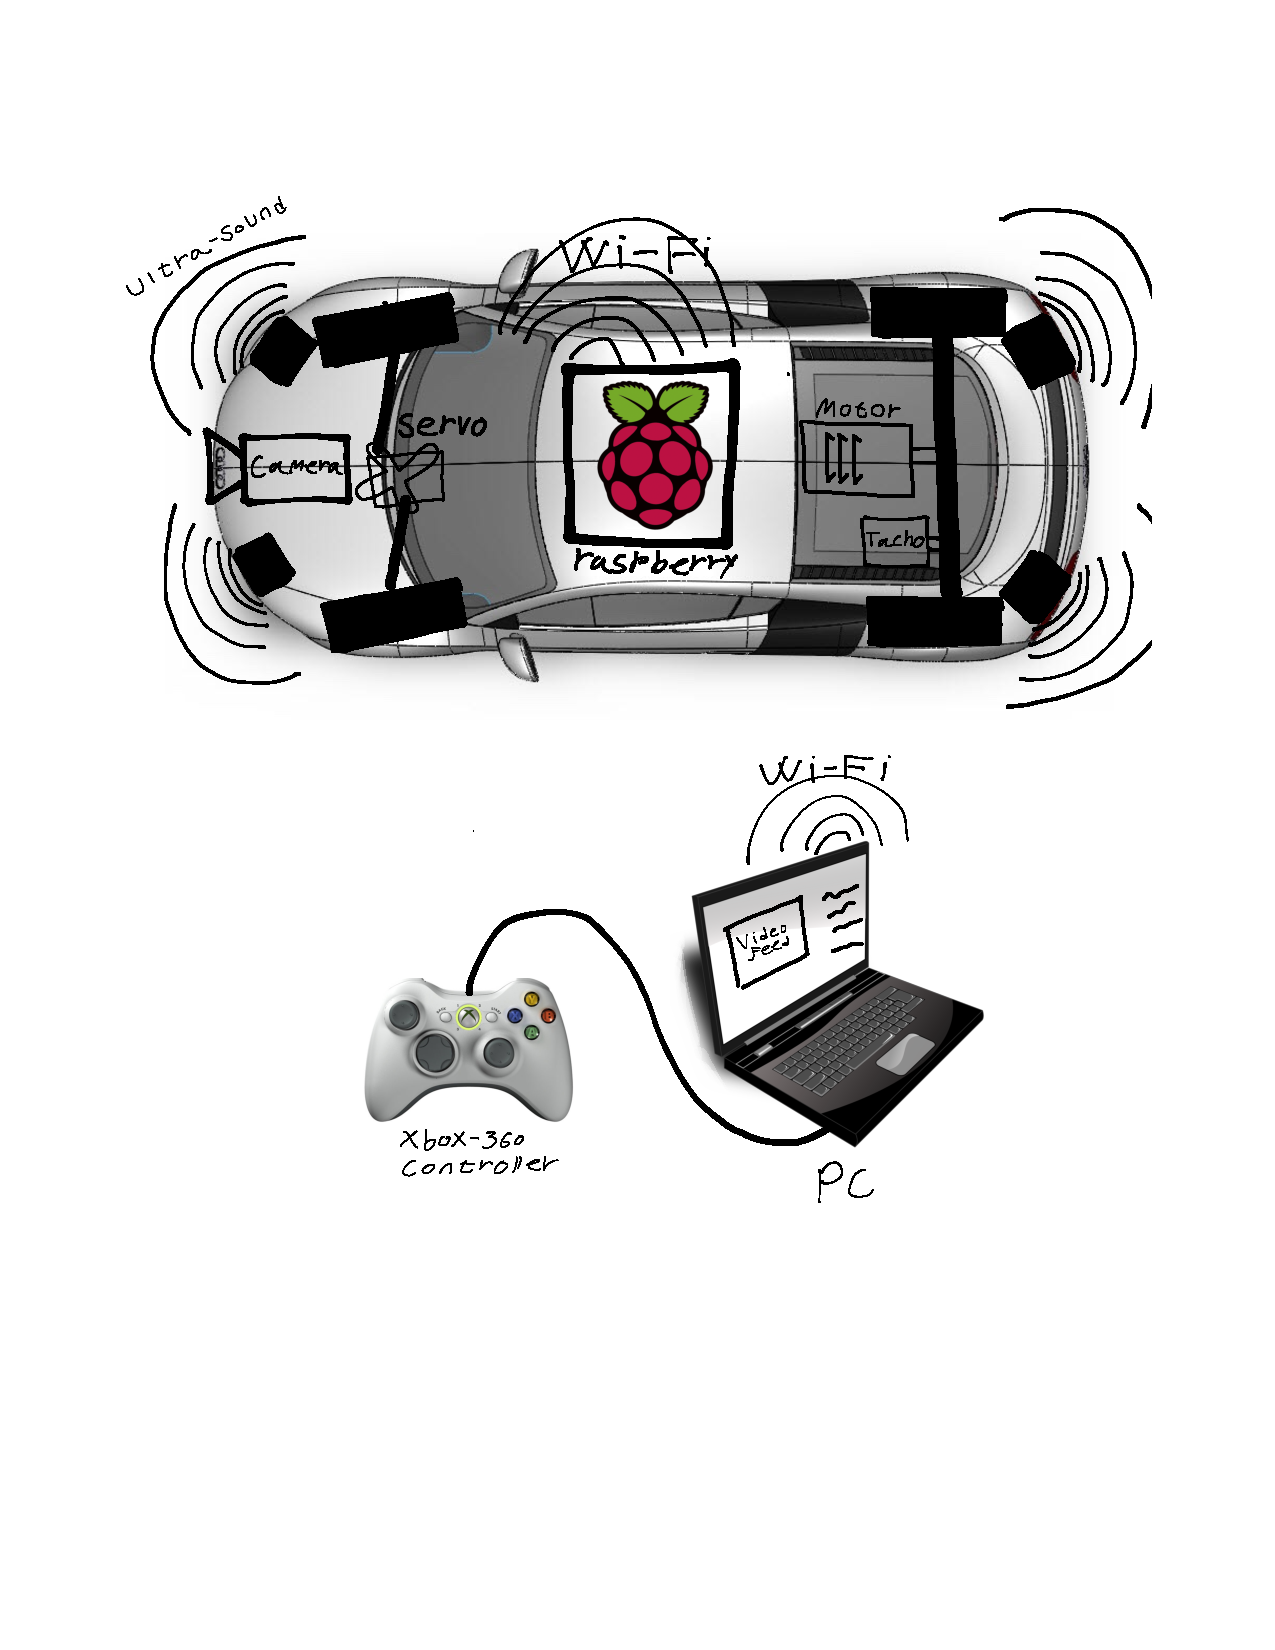
\includegraphics[width=\textwidth - 7.38 cm]{../fig/billeder/rigbillede}
\caption{Rigt billede af det samlede system}
\label{fig:rigbillede}
\end{figure} 
AKS systemet betår af fire distance sensorer, som er monteret på bilen således de kan detektere forhindringer forud og bagud, samt til hvilken side forhindringen er til. På denne måde kan bilen vide om den skal dreje til højre eller venstre, for at undgå en kollision. Forhjulene styres med en servomotor, som ændrer forhjulenes position, når brugeren ændrer positionen af venstre styrepind på Xbox-360 controlleren. Motoren regulerer bilens hastighed ved hjælp af tachometeret således maksimal acceleration altid opnås, når brugeren ændrer positionen af knapperne \texttt{RT} eller \texttt{LT} på controlleren. Hvis brugeren trykker på \texttt{X} bremser bilen. På GUI'et præsenteres data i de lysegrå felter. De mørkegrå felter er knapper som brugeren kan trykke på for hhv. at indstille bilens makshastighed, konfigurere IP-adressen til bilen, oprette forbindelse, kalibrere styretøj, tænde eller slukke for AKS eller for at lukke systemet ned. Se figur \ref{fig:main_menu}. Når brugeren starter GUI'et indtaster brugeren bilens IP-adresse ved at klikke på \texttt{''Konfigurer IP''}. Herefter oprettes forbindelsen til bilen ved at brugeren trykker på \texttt{''Opret forbindelse''}. Når GUI'en har oprettet forbindelse til bilen vises der et video-stream og brugeren ser en meddelelsesboks hvori der gives besked om at forbindelsen er oprettet. Brugeren kan nu manøvrere bilen efter sit ønske, eller benytte GUI'ets muligheder for at indtaste en makshastighed, tænde eller slukke for AKS systemet. For at brugeren altid kan sikre sig bilen kører lige ud, når venstre styrepind på Xboc-360 controlleren står i midterpositionen, kan brugeren indtaste en kalibreringsværdi som gør at bilen selv tager højde for en eventuelt skævhed i styretøjet.

\begin{figure}[h]
\centering
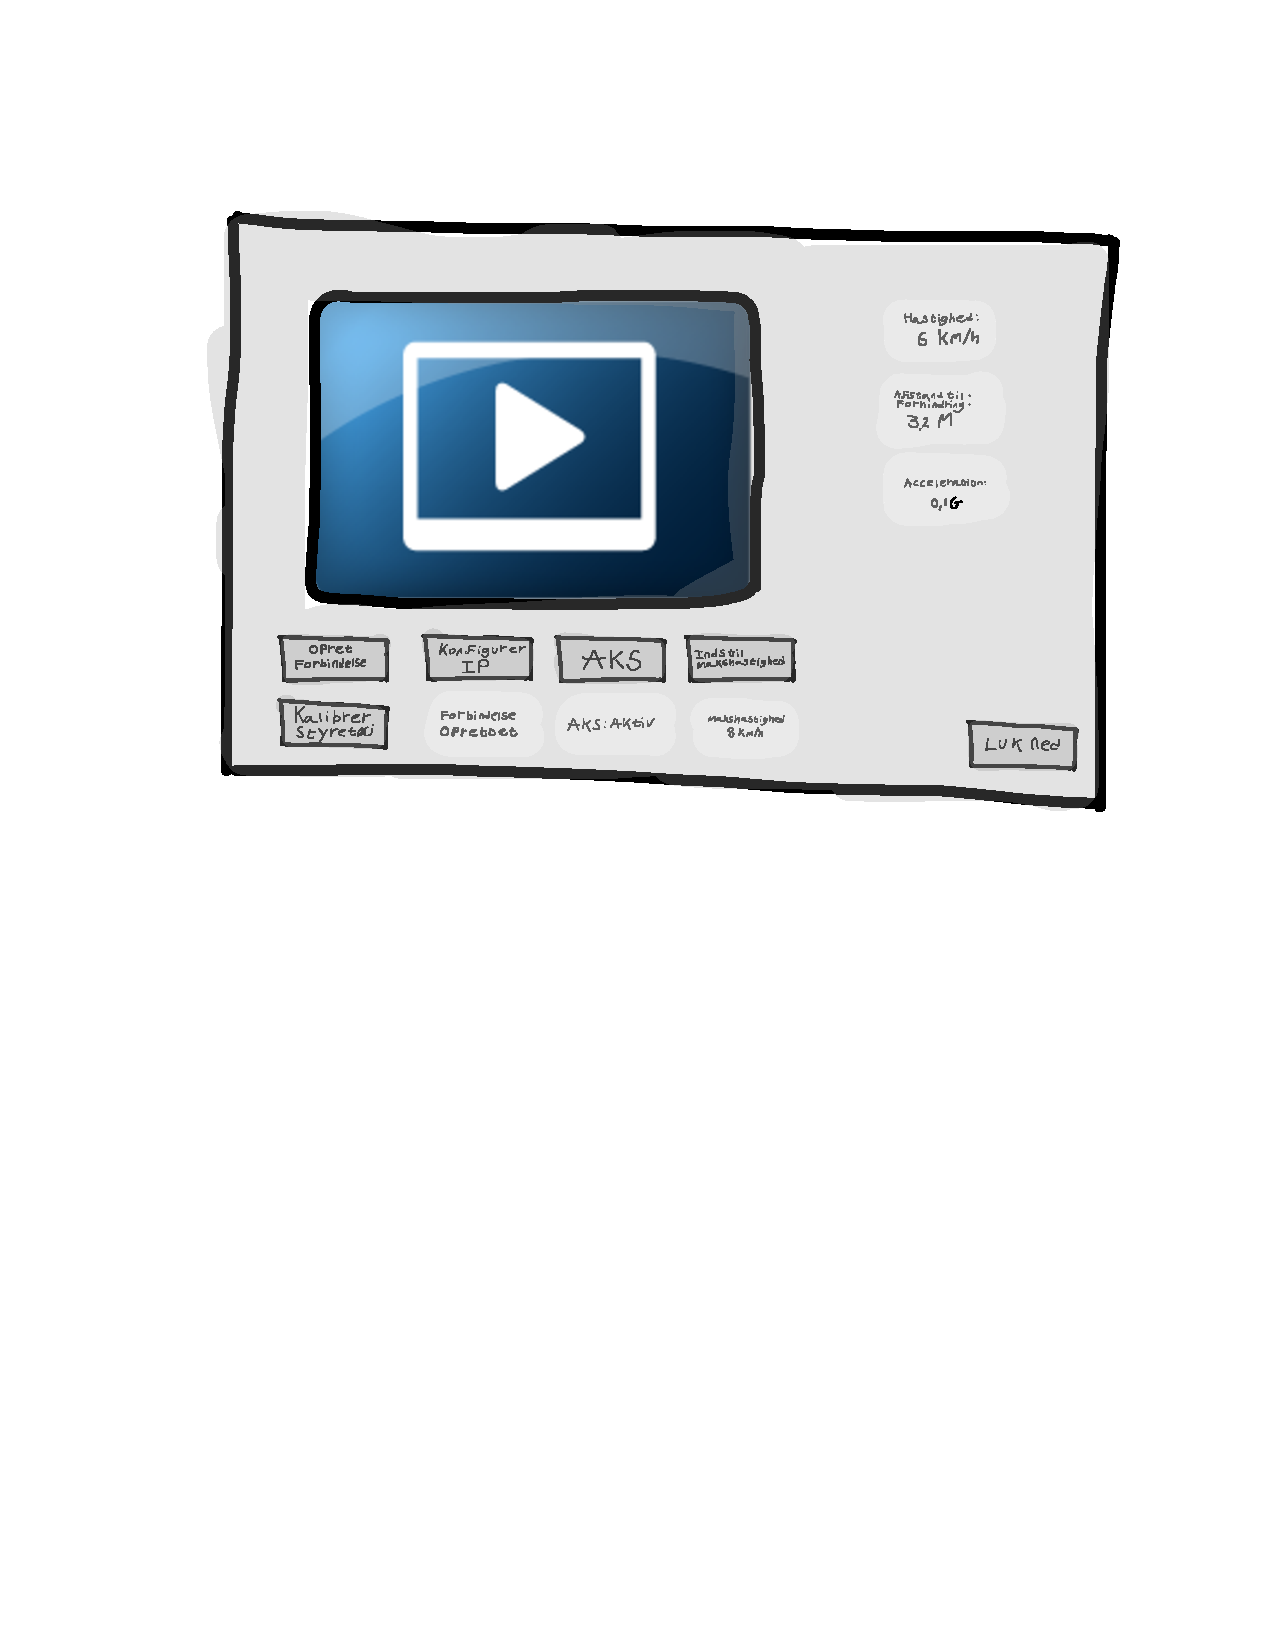
\includegraphics[width=\textwidth*2/3]{../fig/gui/hovedmenu}
\caption{Skitse af hovedmenu}
\label{fig:main_menu}
\end{figure}
